\documentclass[
	12pt,				% tamanho da fonte
	openright,			% capítulos começam em pág ímpar (insere página vazia caso preciso)
	oneside,			% para impressão em recto e verso. Oposto a oneside
	a4paper,			% tamanho do papel. 
	english,			% idioma adicional para hifenização
	french,				% idioma adicional para hifenização
	spanish,			% idioma adicional para hifenização
	brazil				% o último idioma é o principal do documento
	]{abntex2}

\usepackage{lmodern}			% Usa a fonte Latin Modern			
\usepackage[T1]{fontenc}		% Selecao de codigos de fonte.
\usepackage[utf8]{inputenc}		% Codificacao do documento (conversão automática dos acentos)
\usepackage{indentfirst}		% Indenta o primeiro parágrafo de cada seção.
\usepackage{color}				% Controle das cores
\usepackage{graphicx}			% Inclusão de gráficos
\usepackage{microtype} 			% para melhorias de justificação
\usepackage{transparent}
\usepackage{eso-pic}
\usepackage{amsthm,amsfonts}
\usepackage{float}
\usepackage{multirow}
\usepackage[table,xcdraw]{xcolor}
\usepackage{longtable}
\usepackage{lipsum}				% para geração de dummy text
%\usepackage[brazilian,hyperpageref]{backref}	 % Paginas com as citações na bibl
\usepackage[alf]{abntex2cite}	% Citações padrão ABNT
\usepackage{xcolor}
\usepackage{scalefnt}

\usepackage[font=small]{caption}     %% make caption in normal size
\usepackage{etoolbox}
\AtBeginEnvironment{longtabu}{\footnotesize}{}{}   %% change all longtabu content to foot note size

\definecolor{verde}{rgb}{0,0.5,0}
\usepackage{listings}
\lstset{
  language=C++,
  basicstyle=\ttfamily\small,
  keywordstyle=\color{blue},
  stringstyle=\color{verde},
  commentstyle=\color{red},
  extendedchars=true,
  showspaces=false,
  showstringspaces=false,
  numbers=left,
  numberstyle=\tiny,
  breaklines=true,
  backgroundcolor=\color{green!10},
  breakautoindent=true,
  captionpos=b,
  xleftmargin=0pt,
}


\titulo{Modelagem e simulação de uma fábrica de chocolate para definição de layout}
\autor{Gabriel Rodrigues Munhoz 106802\\Vinícius Bertanha Perondi 107422}
\local{Maringá, PR}
\data{11.04.2022}
\orientador{}
\coorientador{}
\instituicao{%
  Universidade Estadual de Maringá - UEM
  \par
  Departamento de Engenharia de Produção - DEP}
\tipotrabalho{Tese (Doutorado)}
\preambulo{}

\definecolor{blue}{RGB}{41,5,195}

\makeatletter
\hypersetup{
     	%pagebackref=true,
	pdftitle={\@title}, 
	pdfauthor={\@author},
    	pdfsubject={\imprimirpreambulo},
	pdfcreator={LaTeX with abnTeX2},
	pdfkeywords={abnt}{latex}{abntex}{abntex2}{trabalho acadêmico}, 
	colorlinks=true,       		% false: boxed links; true: colored links
    	linkcolor=black,          	% color of internal links
    	citecolor=black,        		% color of links to bibliography
    	filecolor=magenta,      		% color of file links
	urlcolor=blue,
	bookmarksdepth=4
}

\setlength{\parindent}{1.3cm}

\setlength{\parskip}{0.2cm}  % tente também \onelineskip

\makeindex

%\usepackage{fancyhdr}
%\fancyhead{}
%\fancyfoot{}
%\lhead{Processo Agroindustrial de Processamento de Cacau}
%\rhead{Processo Agroindustrial de Processamento de Cacau}

\AddToShipoutPicture{
\put(0,0){
\parbox[b][\paperheight]{\paperwidth}{%
\vfill
\centering
{\transparent{0.1}\includegraphics[scale=1.4]{../../Pictures/logoUEM.jpg}    }%
\vfill}}}



%\graphicspath{{../Pictures}}
\begin{document}

\begin{minipage}[c][0cm][c]{0cm} % a primeira minipágina tem uma altura de 1.5cm e uma largura de 3cm.

\centering


\includegraphics[scale=0.45]{../../Pictures/uem-modelo-04.png}  
\end{minipage}

\selectlanguage{brazil}

\frenchspacing 

% \pretextual

\imprimircapa


% ---
% RESUMOS
% ---

%\setlength{\absparsep}{18pt} % ajusta o espaçamento dos parágrafos do resumo
%\begin{resumo}
 
 
% \textbf{Palavras-chave}: latex. abntex. editoração de texto.
%\end{resumo}


% ---
% inserir o sumario
% ---
\pdfbookmark[0]{\contentsname}{toc}
\tableofcontents*
\cleardoublepage

% ----------------------------------------------------------
% ELEMENTOS TEXTUAIS
% ----------------------------------------------------------
\textual

\chapter{Introdução}
%\pagestyle{fancy}

O atual cenário competitivo tem tido grandes atualizações e renovações, afetando, majoritariamente, empresas de pequeno e médio porte, ocasionado pela crescente globalização dos mercados, há uma maior exigência de parâmetros de qualidade, menor prazo de entrega e grandes níveis de customização. 

Para que o cenário fique adequado, as organizações adotam a utilização de ferramentas e técnicas para ampliar a capacidade de tomada de decisão \cite{ESPOSITO}.

Segundo Fernandes (2008), quanto maior a intensidade competitividade no mercado, é maior a necessidade das empresas industriais em tomar decisões mais precisas no respeito aos ajustes e melhorias dos seus sistemas produtivo. O autor afirma que as empresas devem utilizar a simulação computacional como forma de adquirir e organizar o conhecimento necessário para a tomada de decisão.

É possível definir o processo de modelagem e simulação como uma experimentação computacional, onde podemos usar modelos de um sistema real ou sistemas idealizados para o estudo de problemas reais e complexos, com a função de testar diferentes alternativas para encontrar e propor melhores formas de operação que achem a otimização do sistema como um todo. 

As atividades do processo de modelagem e simulação são resumidas conforme esquema mostrado na figura \ref{figfluxo}, iniciado pela construção do modelo, passando pela transformação de modelo conceitual em modelo computacional e chegando aos testes experimentais (simulação propriamente dita).

\begin{figure}[H]
\begin{center}
\caption{Fluxograma do processo de modelagem e simulação resumido}
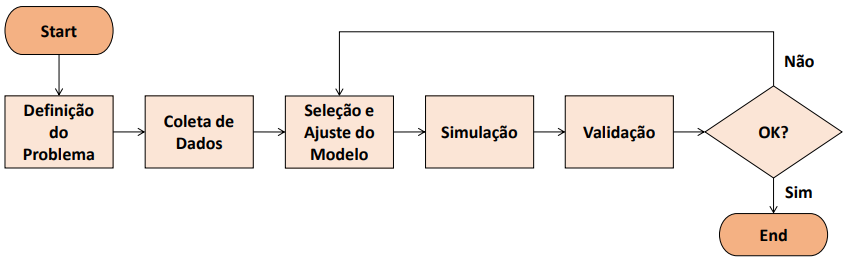
\includegraphics[scale=0.5]{../../Pictures/simulacaoresumida.png} 
\label{figfluxo}
\legend{Fonte: \cite{modelagem}}
\end{center}
\end{figure}

\section{Objetivo Geral}

O objetivo geral deste trabalho é achar a solução do melhor layout do sistema produtivo de uma fábrica de chocolate, atingindo a demanda de 20 toneladas por mês e conferir a representatividade dessas mudanças por intermédio de um modelo de simulação para identificação de atividades críticas e otimização desses sistemas.


%\newpage
\chapter{Revisão Bibliográfica}
%\pagestyle{fancy}

Segundo \cite{Miyagi}, realizar a simulação de processos produtivos é compreendida como a cópia de um processo do mundo real. Ela, a simulação, é uma eficiente ferramenta no aspecto do desenvolvimento de sistemas. 

Na era digital, é possível construir modelos e remodelar sistemas em um pequeno espaço de tempo. Usando a simulação, é viável analisar hipóteses sem a necessidade de testar no mundo real \cite{bateman}. 

O desenvolvimento científico nas tecnologias de simulação vem ganhando mais espaço e importância na formação de profissionais nas áreas da engenharia, em especial na formatação de layouts e linha de produção.

Há algum tempo, a estabilidade da demanda era ganho pelas empresas baseado na exclusividade tecnológica de produção empregada e, também, na procura do mercado consumidor \cite{wang}. 

Portanto, nessa situação, a estratégia competitiva que é selecionada pela maioria das empresas era a de produzir em massa, permitindo a maior redução nos custos fixos. Em vista dos clientes, eles se mantinham satisfeitos com a redução de custo obtida pela estratégia escolhida: muito volume produzido resultando em redução dos preços finais.

No entanto, dentro das últimas décadas, os sistemas de produção foram se tornando cada vez mais complexos para atender aos requisitos da crescente demanda de qualidade e flexibilidade da produção \cite{popovics}. 

Dentro de um ambiente dinâmico, é necessário que suas organizações procurem novas técnicas para planejar com objetivo de melhorar a qualidade dos serviços prestados e produtos entregues \cite{junior}.

Nessa mesma  ordem, segundo Schlegel e Murray (2010), com objetivo de ampliar a capacidade da tomada de decisão, é preciso o desenvolvimento de métodos probabilísticos, para simular a variabilidade das incertezas que o mercado apresenta, normalmente na forma de modelos de apoio para a tomada de decisão.

Levando em consideração a fabricação de chocolate na simulação, o contexto da nossa principal matéria prima, o Cacau, seguem a contextualização: 

O cacau é um fruto da espécie Theobroma cacao L. que possui origem na região amazônica e seu uso, segundo arqueólogos equatorianos e franceses, já era realizado há cerca de 5.500 anos pelos povos amazônicos \cite{unesco}. No entanto, foi no século XVII que acabou se tornando um produto agrícola e cultivado em diferentes locais da América do Sul e Central devido à disseminação do cultivo pelos espanhóis, e posteriormente se expandindo aos poucos pelo mundo. \cite{senar} 

Existem 6 principais produtos a partir do fruto de cacau: mel, polpa, nibs, chocolate, manteiga e cacau em pó, além da própria amêndoa do cacau e casca que também pode ser comercializada de uma forma menos processada. A maior parte desses produtos são voltados para o setor alimentício, no entanto é possível verificar aplicações também no setor cosmético e no setor de geração de energia \cite{hansen}. Com mais da metade da produção nacional, 62$\%$, o sul da Bahia é a principal região produtora de cacau, seguida pela região norte do Brasil com 34$\%$ e o restante da produção, 4$\%$, espalhada pelo país \cite{senar}. O Brasil é o 7º maior produtor do mundo e segundo o Instituto Brasileiro de Geografia Estatística (IBGE) o Brasil produziu em torno de 310 mil toneladas. \cite{Icco} 


%\newpage
\chapter{Metodologia}
%\pagestyle{fancy}

Para fins de estudo sobre o tema de modelagem e simulação, o presente trabalho teve como foco uma pesquisa exploratória. A empresa utilizada para a prática do trabalho é fictícia, contudo foi projetada de forma realista e a complexidade de maquinários e processos são comparáveis com os de empresas reais do mesmo ramo. 

\section{Contextualização da empresa utilizada}

A empresa projetada é uma fábrica de chocolate capaz de produzir 20 toneladas de chocolate ao mês, dimensionada para atender 0,05$\%$ do consumo brasileira de chocolate. A companhia tem em seu portfólio 4 tipos de chocolate: amargo, amargo maturado, meio-amargo e ao leite. 

A linha de produção da empresa possui diversos processos e se encontra de forma mais detalhada no fluxograma da imagem \ref{fluxocacau}.


\begin{figure}[H]
\begin{center}
\caption{Fluxograma do processo de produção de chocolate}
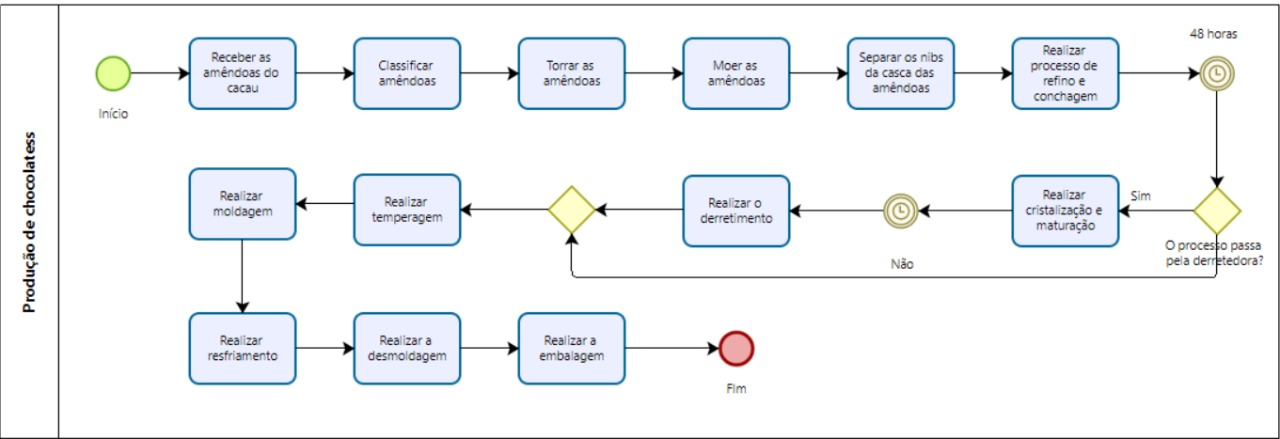
\includegraphics[scale=0.34]{../../Pictures/fluxo1.jpeg} 
\label{fluxocacau}
\legend{Fonte: Autoria Própria}
\end{center}
\end{figure}

E as máquinas que são utilizadas em cada um dos processos foram listadas nas tabelas abaixo:

\newpage

{\fontsize{7.7}{10}\selectfont
\begin{center}
\begin{longtable}[c]{|
>{\columncolor[HTML]{EFEFEF}}l |c|c|cc|c|}
\caption{Informações de maquinários, temperaturas, tempos e perdas de cada etapa do processo}
\label{table6}\\
\hline
\multicolumn{1}{|c|}{\cellcolor[HTML]{EFEFEF}} &
  \cellcolor[HTML]{EFEFEF} &
  \cellcolor[HTML]{EFEFEF} &
  \multicolumn{2}{c|}{\cellcolor[HTML]{EFEFEF}\textbf{Temperaturas (ºC)}} &
  \cellcolor[HTML]{EFEFEF} \\ \cline{4-5}
\multicolumn{1}{|c|}{\multirow{-2}{*}{\cellcolor[HTML]{EFEFEF}\textbf{Etapas}}} &
  \multirow{-2}{*}{\cellcolor[HTML]{EFEFEF}\textbf{Máquina}} &
  \multirow{-2}{*}{\cellcolor[HTML]{EFEFEF}\textbf{Tempo (h)}} &
  \multicolumn{1}{c|}{\cellcolor[HTML]{EFEFEF}\textbf{Entrada}} &
  \cellcolor[HTML]{EFEFEF}\textbf{Saída} &
  \multirow{-2}{*}{\cellcolor[HTML]{EFEFEF}\textbf{Perdas}} \\ \hline
\endhead
%
\textbf{1. Classificação} &
  - &
  0,20 &
  \multicolumn{1}{c|}{25 - 29 (a)} &
  25 - 29 (a) &
  2\% \\ \hline
\textbf{2. Torrefação} &
  Torrador industrial &
  0,50 &
  \multicolumn{1}{c|}{25 - 29 (a)} &
  110 &
  5\% \\ \hline
\textbf{3. Moagem} &
  Moedor industrial &
  0,40 &
  \multicolumn{1}{c|}{110} &
  25 - 29 (a) &
  2\% \\ \hline
\textbf{4. Descasque} &
  Descascador de amêndoas &
  0,40 &
  \multicolumn{1}{c|}{25 - 29 (a)} &
  25 - 29 (a) &
  12\% \\ \hline
\textbf{5. Refino + Conchagem} &
  Melanger &
  48,00 &
  \multicolumn{1}{c|}{25 - 29 (a)} &
  50 &
  4\% \\ \hline
\textbf{6. Cristalização} &
  - &
  0,50 &
  \multicolumn{1}{c|}{50} &
  25 - 29 (a) &
  1\% \\ \hline
\textbf{7. Maturação} &
  - &
  \multicolumn{1}{l|}{1440,00 - 8760,00} &
  \multicolumn{1}{c|}{25 - 29 (a)} &
  25 - 29 (a) &
  2\% \\ \hline
\textbf{8. Derretimento} &
  Derretedeira de chocolate &
  0,50 &
  \multicolumn{1}{c|}{25 - 29 (a)} &
  42 &
  2\% \\ \hline
\textbf{9. Temperagem} &
  Temperadeira &
  0,35 &
  \multicolumn{1}{c|}{35} &
  28 &
  2\% \\ \hline
\textbf{10. Moldagem} &
  Dosadora + Mesa vibratória &
  0,35 &
  \multicolumn{1}{c|}{28} &
  25 - 29 (a) &
  1\% \\ \hline
\textbf{11. Resfriamento} &
  Túnel de resfriamento &
  0,50 &
  \multicolumn{1}{c|}{25 - 29 (a)} &
  12 &
  0\% \\ \hline
\textbf{12. Desmolde} &
  - &
  0,35 &
  \multicolumn{1}{c|}{12} &
  20 &
  1\% \\ \hline
\textbf{13. Embalagem} &
  Embaladora &
  0,50 &
  \multicolumn{1}{c|}{20} &
  20 &
  1\% \\ \hline
\end{longtable}
\centering \footnotesize{Fonte: Autoria própria}
\end{center}
}

{\fontsize{7}{10}\selectfont
\begin{center}
\begin{longtable}[c]{|
>{\columncolor[HTML]{EFEFEF}}c |c|c|c|c|c|c|}
\caption{Maquinário detalhado}
\label{maquina}\\
\hline
\textbf{Máquina} &
  \cellcolor[HTML]{EFEFEF}\textbf{\begin{tabular}[c]{@{}c@{}}Dimensões\\ (AxLxP) (m)\end{tabular}} &
  \cellcolor[HTML]{EFEFEF}\textbf{\begin{tabular}[c]{@{}c@{}}Potência\\ (kW)\end{tabular}} &
  \cellcolor[HTML]{EFEFEF}\textbf{Capacidade} &
  \cellcolor[HTML]{EFEFEF}\textbf{Material} &
  \cellcolor[HTML]{EFEFEF}\textbf{\begin{tabular}[c]{@{}c@{}}Setup\\ (min)\end{tabular}} &
  \cellcolor[HTML]{EFEFEF}\textbf{Especificações} \\ \hline
\endhead
%
\textbf{Torrador industrial} &
  1,8 x 1,4 x 1,4 &
  8,0 &
  10,0 (kg) &
  - &
  15 &
  - \\ \hline
\textbf{Moedor industrial} &
   &
   &
   &
   &
   &
   \\ \cline{1-1}
\textbf{Descascador de amêndoas} &
  \multirow{-2}{*}{1,3 x 0,8 x 1,3} &
  \multirow{-2}{*}{2,2} &
  \multirow{-2}{*}{10 (kg)} &
  \multirow{-2}{*}{Inox} &
  \multirow{-2}{*}{90} &
  \multirow{-2}{*}{400 kg/h} \\ \hline
\textbf{Melanger*} &
  1,2 x 0,7 x 0,7 &
  0,75 &
  100,0 (kg) &
  \begin{tabular}[c]{@{}c@{}}Inox 304 e \\ Granito Cinza\end{tabular} &
  30 &
  - \\ \hline
\textbf{Compressor de ar} &
  0,3 x 0,6 x 0,6 &
  1,5 &
  25,0 (l) &
  - &
  - &
  - \\ \hline
\textbf{Derretedeira de chocolate} &
  0,7 x 0,6 x 0,4 &
  7,5 &
  50,0 (kg) &
  Inox 304 &
  60 &
  - \\ \hline
\textbf{Temperadeira} &
  0,7 x 0,5 x 0,6 &
  2,9 &
  100,0 (kg) &
  Inox 304 &
  60 &
  5 kg a cada 8min \\ \hline
\textbf{Dosadora (Ø30)} &
  1,5 x 1,1 x 1,4 &
  0,02 &
  100,0 (l) &
  Inox &
  60 &
  \begin{tabular}[c]{@{}c@{}}8 pistões - 50g/pistão\\ 20 ciclos/min\end{tabular} \\ \hline
\textbf{Mesa vibratória*} &
  0,7 x 1,1 x 0,6 &
  0,2 &
  - &
  Inox 304 &
  10 &
  - \\ \hline
\textbf{Túnel de resfriamento} &
  1,2 x 0,6 x 9,0 &
  5,4 &
  - &
  Inox 304 &
  20 &
  - \\ \hline
\textbf{Embaladora} &
  3,3 x 2,9 x 1,4 &
  3,1 &
  - &
  - &
  20 &
  350 pacotes/min \\ \hline
\end{longtable}
*Máquinas que utilizam Compressor de ar \\
\centering \footnotesize{Fonte: Autoria própria}
\end{center}
}

A empresa foi projetada para estar em Belo Horizonte, MG, e os galpões que foram dimensionados para a companhia giram em torno de 800m² de área utilizável.

\begin{figure}[H]
\begin{center}
\caption{Dimensionamento dos máquinas}
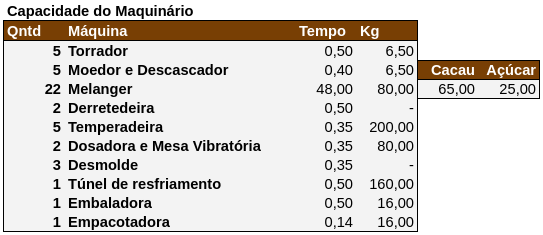
\includegraphics[scale=0.9]{/home/grmunhoz/Documents/Munhoz/University/UEM/Simulacao/Maquinario.png} 
\legend{Fonte: Autoria própria}
\label{maq}
\end{center}
\end{figure}

\begin{figure}[H]
\begin{center}
\caption{Dimensionamento dos colaboradores}
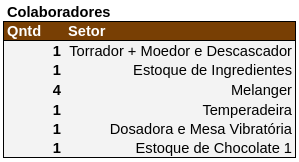
\includegraphics[scale=1]{/home/grmunhoz/Documents/Munhoz/University/UEM/Simulacao/Colaboradores.png} 
\legend{Fonte: Autoria própria}
\end{center}
\end{figure}

\section{Metodologia utilizada para modelagem e simulação}

Com esse conhecimento sobre a companhia utilizada para estudo, o trabalho seguiu as etapas da figura \ref{fluxo}. Esse fluxograma, elaborado por Bateman et al. (2013), abrange todas as fases de um processo de modelagem e simulação de uma empresa é iterativo, o que o torna muito assertivo se utilizado de forma correta.

\begin{figure}[H]
\begin{center}
\caption{Fluxograma do processo de modelagem e simulação completo}
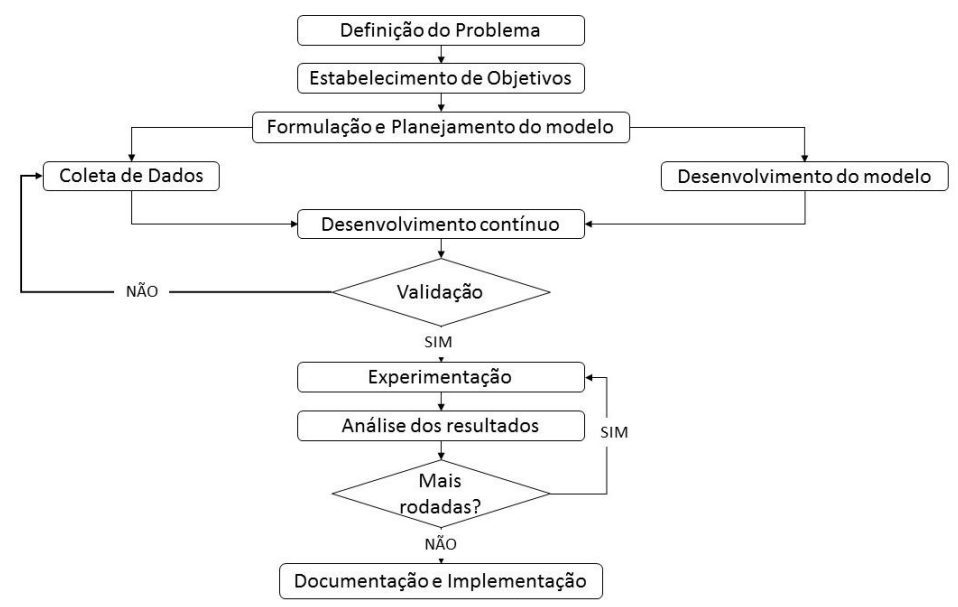
\includegraphics[scale=0.45]{../../Pictures/bateman.png} 
\label{fluxo}
\legend{Fonte: \cite{bateman}}
\end{center}
\end{figure}

\subsection{Definição do Problema}
	
A definição do problema é a primeira etapa da modelagem e é a partir dela que o estudo consegue focar e começar a mapear tudo que pode estar envolvido com aquele problema. Neste trabalho o problema que será estudado será a definição do layout da empresa.

\subsection{Objetivos}
		
Após a definição do problema, são listados os objetivos que são os primeiros passos para a quantificação do problema selecionado. Nessa fase é importante entender no que o problema estudado impacta, para que assim a simulação tenha um discernimento claro dos melhores resultados. 

Para a análise do layout, um objetivo muito importante é a diminuição do tempo que o produto leva para ser transportado de uma máquina para a outra, pois esse transporte excessivo gera um custo desnecessário. Além disso, outro objetivo deve ser a facilidade de carga e descarga de mercadoria, assim como a facilidade de manutenção e operação de qualquer um dos equipamentos.

\subsection{Formulação de planejamento do modelo}

Nessa etapa foi realizado o planejamento do modelo. Para realização da simulação será utilizado o software FlexSim por ser de fácil utilização e com grande capacidade de personalização, além da capacidade de gerar gráficos que auxiliam a tomada de decisão. Nessa etapa foi realizado o desenvolvimento no software e todos os parâmetros utilizados.

\begin{figure}[H]
\begin{center}
\caption{Interface do software FlexSim}
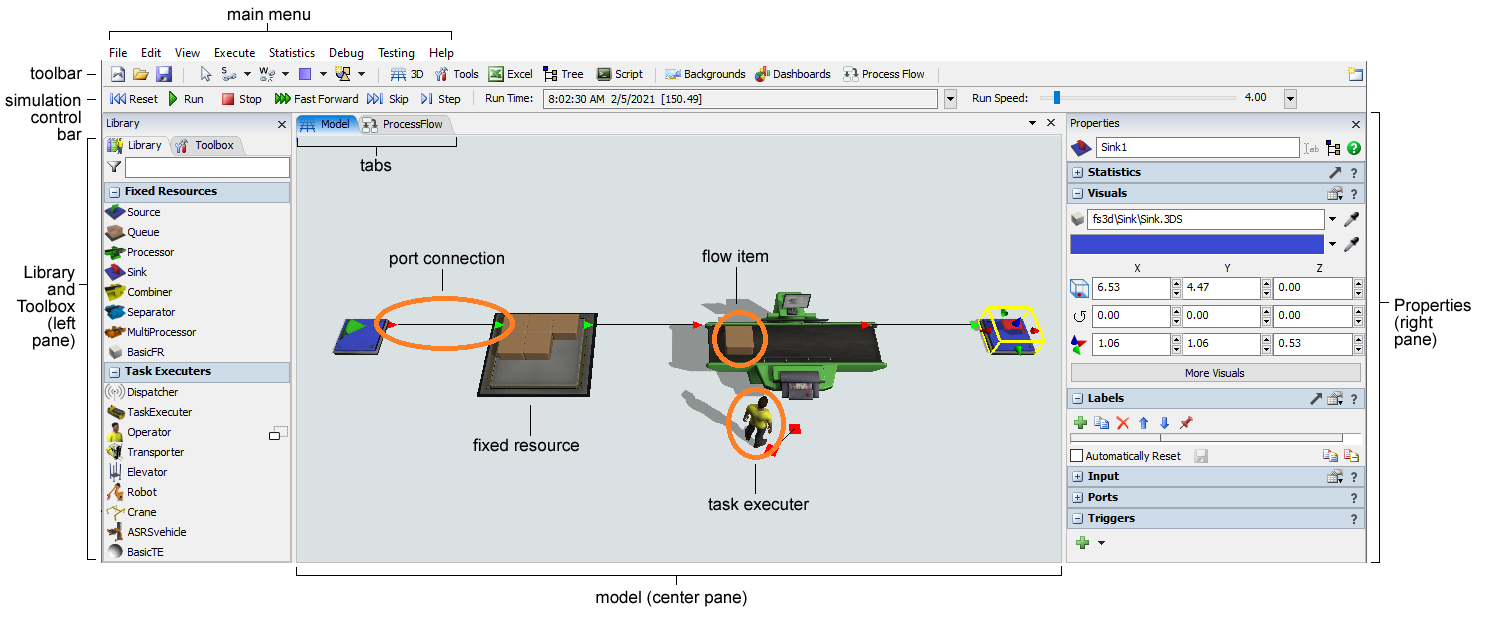
\includegraphics[scale=0.4]{../../Pictures/interface.png} 
\label{fluxo}
\legend{Fonte: \cite{flexsim}}
\end{center}
\end{figure}


Para a construção do layout no simulador FlexSim foram estabelecidas as necessidades dos estoques estarem próximos da saída do galpão e a proximidade das máquinas que são sequenciais no processo de fabricação do chocolate. Além disso, foram definidos os tipos de processadores que são utilizados no programa e que a movimentação entre eles são feitos principalmente por meio de esteiras, contudo a movimentação da esteira para as máquinas são realizadas por colaboradores.

\subsection{Coleta de dados e desenvolvimento do modelo}

Segundo, Bateman et al. as fases de coleta de dados e desenvolvimento do modelo são fundamentais para que os resultados sejam realistas e possam ser utilizados. Neste momento a modelagem já se torna mais robusta e complexa de acordo com a quantidade de dados que será utilizada no modelo. Ademais, é nessa etapa que ocorre já o começo da simulação com o desenvolvimento do modelo no software escolhido.

Durante essa fase o projeto focou em desenvolver toda a simulação no software com todas as especificações e capacidades das máquinas, além da divisão dos colaboradores por setores.



\subsection{Validação}

	A validação também é de extrema importância para a simulação, pois com ela é possível averiguar se o modelo simulado consegue de forma precisa reproduzir com grande fidelidade a linha de produção que foi projetada. São realizados muitos testes de validação e comparações entre os resultados esperados do mundo real e os resultados obtidos a partir da simulação. Nesse momento é de grande importância a presença de especialistas no assunto para que eles consigam detalhar melhor todo o funcionamento que normalmente existe.

	A simulação que foi feita neste trabalho, no entanto, não realizou essa fase já que ela possui caráter mais exploratório e não se trata de um estudo de caso real. 

\subsection{Experimentação}

	Nessa etapa, ocorre a criação de cenários de simulação, estes serão os responsáveis pelos diferentes resultados da simulação. Cada cenário é uma solução para o problema estudado e em cada um deles são definidas algumas variáveis que modificam o resultado final e impactam nos indicadores que são utilizados para tomada de decisão.

	Para o estudo do layout, as principais variáveis são as coordenadas de localização das máquinas e esteiras, pois essas distâncias entre as coordenadas influenciam no tempo de transporte dos itens. Assim, cada cenário teve um conjunto de localizações específicas para cada objeto relevante da linha de produção, e a partir desses cenários foram calculados os indicadores: distância percorrida pelos colaboradores e análise financeira. 

\subsection{Análise dos resultados}

Por fim, com os resultados das experimentações foi possível analisar e verificar qual foi o melhor cenário e as possíveis causas desses resultados. Nesta última fase, os gráficos e tabelas foram de grande auxílio e puderam tornar a visualização dos resultados mais claras. O uso do dashboard do FlexSim nesse caso foi de grande ajuda, pois possibilitou a criação de diversos gráficos que foram utilizados para escolha dos melhores cenários.

\chapter{Análise dos Resultados}

Seguindo com o objetivo do projeto, foram simulados dois diferentes cenários, ambos com o mesmo número de colaboradores (9) e maquinários (44). A simulação foi feita para um período de 30 dias, sendo que a linha de produção trabalhava 8 horas diárias todos os dias, e com os dados coletados pelo Software FlexSim foi gerado um gráfico de distância percorrida pelos colaboradores e uma análise financeira.


\section*{Layout 1}

\begin{figure}[H]
\begin{center}
\caption{Layout 1 no software FlexSim}
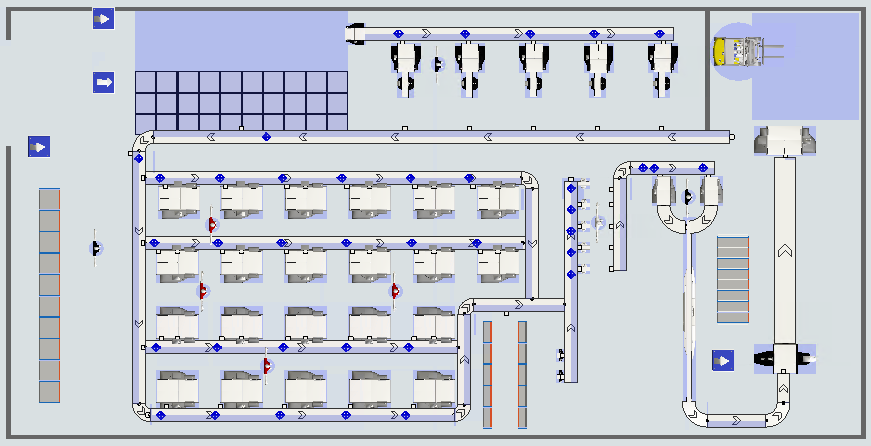
\includegraphics[scale=0.55]{/home/grmunhoz/Documents/Munhoz/University/UEM/Simulacao/Layout1.1.png} 
\legend{Fonte: Autoria Própria}
\end{center}
\end{figure}

\begin{figure}[H]
\begin{center}
\caption{Gráfico da distância percorrida pelos colaboradores do Layout 1}
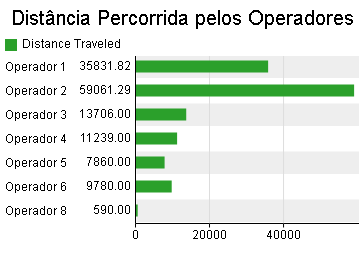
\includegraphics[scale=0.7]{/home/grmunhoz/Documents/Munhoz/University/UEM/Simulacao/DistanciaL1.png} 
\legend{Fonte: Autoria Própria}
\end{center}
\end{figure}

\begin{figure}[H]
\begin{center}
\caption{Resultado financeiro do Layout 1}
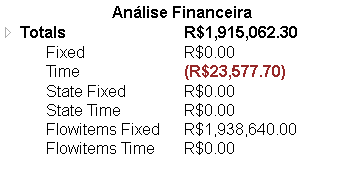
\includegraphics[scale=0.7]{/home/grmunhoz/Documents/Munhoz/University/UEM/Simulacao/FinanceiroL1.png} 
\legend{Fonte: Autoria Própria}
\end{center}
\end{figure}

\section*{Layout 2}

\begin{figure}[H]
\begin{center}
\caption{Layout 2 no software FlexSim}
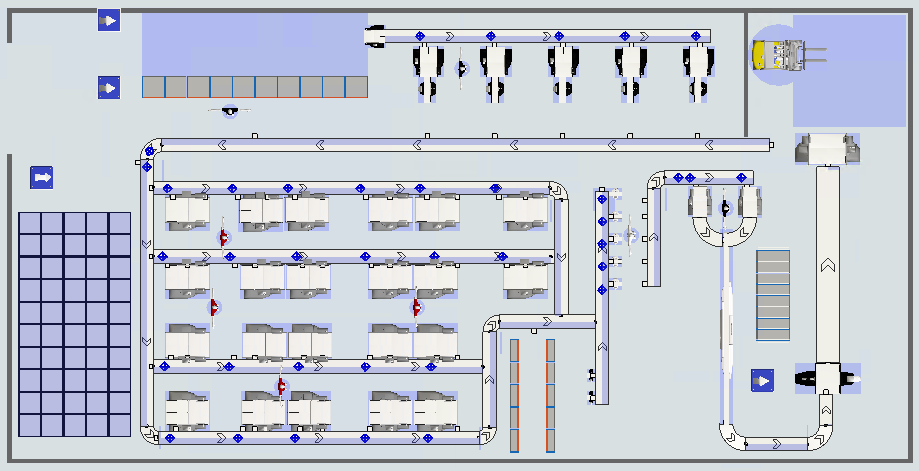
\includegraphics[scale=0.55]{/home/grmunhoz/Documents/Munhoz/University/UEM/Simulacao/Layout2.1.png} 
\legend{Fonte: Autoria Própria}
\end{center}
\end{figure}

\begin{figure}[H]
\begin{center}
\caption{Gráfico da distância percorrida pelos colaboradores do Layout 2}
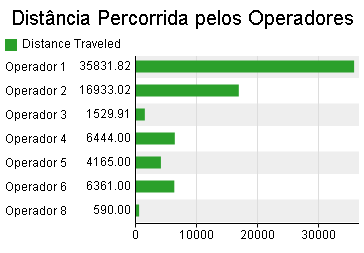
\includegraphics[scale=0.7]{/home/grmunhoz/Documents/Munhoz/University/UEM/Simulacao/DistanciaL2.png} 
\legend{Fonte: Autoria Própria}
\end{center}
\end{figure}

\begin{figure}[H]
\begin{center}
\caption{Resultado financeiro do Layout 2}
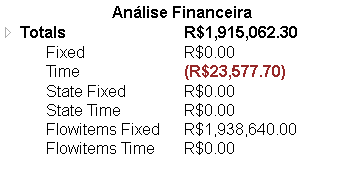
\includegraphics[scale=0.7]{/home/grmunhoz/Documents/Munhoz/University/UEM/Simulacao/FinanceiroL2.png} 
\legend{Fonte: Autoria Própria}
\end{center}
\end{figure}

O Layout 2 permite que os colaboradores realizem menos movimentos, diferença de 66.213,36 metros, e tenha o mesmo desempenho financeiro, R\$1.915.062,30. Nesse layout foram modificadas apenas as localizações das máquinas Melangers e houve a troca do estoque de ingredientes com o estoque de produto final, apenas essas diferenças já foram capazes de influenciar no resultado final, fazendo com que o Layout 2 se tornasse muito mais atrativo para a empresa, pois irá economizar tempo de transporte e também irá cansar menos os funcionários dessa linha de produção. Os detalhes e divisões do Layout 2 podem ser verificados na imagem \ref{detalhado}.

\begin{figure}[H]
\begin{center}
\caption{Layout 2 no software FlexSim}
\includegraphics[scale=0.4]{/home/grmunhoz/Documents/Munhoz/University/UEM/Simulacao/Layout2.2.png} 
\legend{Fonte: Autoria Própria}
\label{detalhado}
\end{center}
\end{figure}

%\newpage
\chapter{Conclusão}
%\pagestyle{fancy}

Portanto, conforme a análise dos dois layouts montados dentro do Software FlexSim, o Layout 2, onde as máquinas estão mais próximas (economizando movimentação dos colaboradores), é o modelo mais efetivo para a fabricação de chocolate nesse linha de produção montada dentro do projeto, o que foi ao encontro do objetivo geral do trabalho que era encontrar uma solução ótima de layout para a fábrica. 

Além disso, a questão exploratória do trabalho também foi atingida com sucesso, já que durante a modelagem e simulação dos 2 cenários no software FlexSim foi possível entender e aprender muito sobre a técnica de simulação.

Por fim, a técnica da simulação para auxiliar nessa tomada de decisão foi de grande ajuda, pois além de possibilitar a montagem de diversos cenários de layout ela possibilitou a visualização de como a fábrica de chocolates funcionaria e como os colaboradores se movimentariam. 

\newpage
\postextual

\bibliography{referencias}

%\begin{anexosenv}

%\chapter{Código utilizado no software EMSO}

%\begin{lstlisting}
%\end{lstlisting}

%\end{anexosenv}

\end{document}